% generated by doc/figures.py -- edit the script, not this file
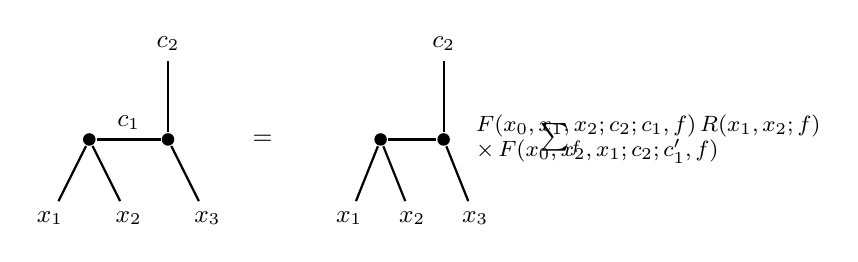
\begin{tikzpicture}[thick, every node/.style={font=\small}]
  \node (x1) at (0,0) {$x_1$};
  \node (x2) at (1.0,0) {$x_2$};
  \node (x3) at (2.0,0) {$x_3$};
  \node[circle, fill, inner sep=1.6pt] (a) at (0.5,1.0) {};
  \node[circle, fill, inner sep=1.6pt] (b) at (1.5,1.0) {};
  \draw (x1) -- (a); \draw (x2) -- (a);
  \draw (a) -- (b) node[midway, above] {$c_1$};
  \draw (x3) -- (b);
  \draw (b) -- (1.5,2.0) node[above] {$c_2$};
  \node at (2.7,1.0) {$=$};
  \node (y1) at (3.8,0) {$x_1$};
  \node (y2) at (4.6,0) {$x_2$};
  \node (y3) at (5.4,0) {$x_3$};
  \node[circle, fill, inner sep=1.6pt] (c) at (4.2,1.0) {};
  \node[circle, fill, inner sep=1.6pt] (d) at (5.0,1.0) {};
  \draw (y1) -- (c); \draw (y2) -- (c);
  \draw (c) -- (d);
  \draw (y3) -- (d);
  \draw (d) -- (5.0,2.0) node[above] {$c_2$};
  \node at (6.5,1.0) {$\sum_{f}$};
  \node[align=left] at (7.6,1.0)
    {\footnotesize $F(x_0,x_1,x_2;c_2;c_1,f)\,R(x_1,x_2;f)$\\[-2pt]
     \footnotesize $\times\,F(x_0,x_2,x_1;c_2;c_1',f)$};
\end{tikzpicture}
